\documentclass{article}
\usepackage[utf8]{inputenc}
\usepackage{amsmath}
\usepackage{listings}
\usepackage{geometry}
\usepackage{graphicx}
\usepackage{subfig}
\usepackage[colorlinks=true]{hyperref}
\title{%
Project 1 - 1-D Poisson Equation \\
\large FYS3150 at University of Oslo}
\author{Simen Løken}
\date{September 2020}
\footskip = 90pt
\topmargin = -40pt
\begin{document}

\maketitle
\section{Abstract}
In this project we're going to be looking at different solutions of the one dimensional Poisson Equation. We're going to be using the Tridiagonal Matrix Algorithm (Thomas Algorithm), both in it's general and a special form uniquely fit to our matrix, and we're going to try brute-forcing a solution using an LU-decomposition, and compare FLOPs and computation time to better understand how we can maximize the efficiency of our programs and the limitations of hardware like memory. We find that we can optimize the general algorithm for and go from 9n FLOPs to 4n.
\section{Introduction}
The Poisson Equation is a flexible equation with a broad range of uses in physics, from electromagnetism to Newtonian gravity. In it's most general form it's given as:
\begin{equation}
    \Delta \varphi = f
\end{equation}
However, for our purposes, the one dimensional variation can be expressed as:
\begin{equation}
    -u'' = f(x)
\end{equation}
To properly solve this problem we've been given, we're going to be using Python. While solving the problem itself is quite trivial, the main objective of this project is to optimize and refine our method. Thus, we're going to be trying and comparing three solutions, a general Thomas Algorithm, a specialized Thomas Algorithm and an LU-decomposition.
\section{Theory and Method}
\subsection{Theory}
Our second order differential equation is given as
\begin{equation}
    \frac{\delta^2 u(x)}{\delta x^2} = f(x)
\end{equation}
with a Dirichlet boundary $$x \in (0,1), u(0)=u(1)=0$$
We assume that the function f(x) is given as:
\begin{equation}
    f(x) = 100e^{-10x}
\end{equation}
which gives us the analytical solution
\begin{equation}
    u(x) = 1-(1-e^{-10})x-e^{-10x}
\end{equation}
Given that we now know f(x) and we're looking to find the second derivative, we can approximate it using a Taylor Expansion. This gives us:
\begin{equation}
   -\frac{v_{i+1}+v_{i-1}-2v_i}{h^2} = f_i  \hspace{0.5cm} \mathrm{for} \hspace{0.1cm} i=1,\dots, n,
\end{equation}
where $h$ is the dynamic step-size given as $h = \frac{1}{n-1}$ given by $n$ points and $v_{i}$ is the discrete form of $u$.
We can rewrite this to fit a matrix. For simplicity and generality, let's rename:
\begin{equation}
   -\frac{a_{i}+c_{i}-2b_{i}}{h^2} = f_i  \hspace{0.5cm} \mathrm{for} \hspace{0.1cm} i=1,\dots, n,
\end{equation}
This can be rewritten as the $n\times n$ matrix
\[
\begin{bmatrix}
                           b_1& c_1 & 0 &\dots   & \dots &\dots \\
                           a_1 & b_2 & c_2 &\dots &\dots &\dots \\
                           & a_2 & b_3 & c_3 & \dots & \dots \\
                           & \vdots   & \vdots &\ddots   &\vdots & \vdots \\
                           &   &  &a_{n-2}  &b_{n-1}& c_{n-1} \\
                           &    &  &   &a_{n-1} & b_n 
            \end{bmatrix} = f_i h^2
\]
We name our matrix $A$ and generalize the equation above to be:
\begin{equation} \label{4}
    \mathbf{A}\mathbf{v}=\mathbf{b}
\end{equation}
where $\mathbf{v}$ are solutions to $\mathbf{b}$ and $\mathbf{b}$ is $h^2f_i$
\subsection{Method}
Like previously mentioned, we're going to be employing a general solution given by the Thomas Algorithm.
For simplicity's sake, let's assume we've got a $5\times 5$ matrix:
\[
\mathbf{A}=\begin{bmatrix}
                           b_1& c_1& 0& 0& 0& \\
                           a_1& b_2& c_2& 0& 0& \\
                           0& a_2& b_3& c_3& 0& \\
                           0& 0& a_3& b_4& c_4& \\
                           0& 0& 0& a_4& b_5& \\
\end{bmatrix}
\]
This gives us $$\mathbf{A}\mathbf{v}=\mathbf{f}$$

\[
\begin{bmatrix}
                           b_1& c_1& 0& 0& 0& \\
                           a_1& b_2& c_2& 0& 0& \\
                           0& a_2& b_3& c_3& 0& \\
                           0& 0& a_3& b_4& c_4& \\
                           0& 0& 0& a_4& b_5& \\
\end{bmatrix}
\begin{bmatrix}
                           v_1&\\
                           v_2&\\
                           v_3&\\
                           v_4&\\
                           v_5&
\end{bmatrix}=
\begin{bmatrix}
                           f_1&\\
                           f_2&\\
                           f_3&\\
                           f_4&\\
                           f_5&
\end{bmatrix}
\]
\break
Which we can rewrite as
\[
\mathbf{A}=\begin{bmatrix}
                           b_1& c_1& 0& 0& 0& f_1&\\
                           a_1& b_2& c_2& 0& 0& f_2&\\
                           0& a_2& b_3& c_3& 0& f_3&\\
                           0& 0& a_3& b_4& c_4& f_4&\\
                           0& 0& 0& a_4& b_5& f_5&\\
\end{bmatrix}
\]
\break
with which we can use Guassian elimination, giving us
\[
\mathbf{A}=\begin{bmatrix}
                           b_1& c_1& 0& 0& 0& f_1&\\
                           a_1& \Tilde{b_2}& c_2& 0& 0& \Tilde{f_2}&\\
                           0& a_2& \Tilde{b_3}& c_3& 0& \Tilde{f_3}&\\
                           0& 0& a_3& \Tilde{b_4}& c_4& \Tilde{f_4}&\\
                           0& 0& 0& a_4& \Tilde{b_5}& f_5&\\
\end{bmatrix}
\]
where $\Tilde{b_i}$ and $\Tilde{f_i}$ are given as:
\begin{equation} \label{1}
    \Tilde{b_i}=b_i-\frac{a_{i-1}\cdot c_{i-1}}{\Tilde{b}_{i-1}}
\end{equation}
\begin{equation}\label{2}
    \Tilde{f_i}=f_i-\frac{a_{i-1}\cdot \Tilde{f}_{i-1}}{\Tilde{b}_{i-1}}
\end{equation}
This is the forward substitution of our method. We've now got to do backwards substitution to finally find $\mathbf{v}$.
For simplicity's sake, we redefine $$f_1 = \Tilde{f_1} \hspace{0.5cm} b_1 = \Tilde{b}_{1}$$
We can now eliminate the upper part of the matrix, which gives us
\begin{equation}\label{3}
    u_i = \frac{\Tilde{f_i}-c_i\cdot u_{i+1}}{\Tilde{b}_{i}}
\end{equation}

We can use this algorithm in Python to solve our problem. The algorithm looks like this:
\begin{lstlisting}[language=Python]
def gen(u,f,n,f_t):
    f_t[1] = f[1]
    for i in range(2,n+1): 
        bV[i] = bV[i]-(aV[i]*cV[i-1])/bV[i-1]
        f_t[i] = f[i] - (aV[i]*f_t[i-1])/bV[i-1]
    u[n] = f_t[n]/bV[n]
    for j in range(n-1,-1,-1):
        u[j] = (f_t[j]-cV[j]*u[j+1])/bV[j]
    return u
\end{lstlisting}
We'll now be looking at the special case. While our solution above works for any tridiagonal matrix, we've not taken advantage of the fact that our matrix $\mathbf{A}$ is symmetrical along the diagonal.
\[
\mathbf{A} = \begin{bmatrix}
                           2& -1& 0 &\dots   & \dots &0 \\
                           -1 & 2 & -1 &0 &\dots &\dots \\
                           0&-1 &2 & -1 & 0 & \dots \\
                           & \dots   & \dots &\dots   &\dots & \dots \\
                           0&\dots   &  &-1 &2& -1 \\
                           0&\dots    &  & 0  &-1 & 2 \\
                      \end{bmatrix}
\]
This means that we can rewrite our previous equations, equation \ref{1} and equation \ref{2}.
Components now cancel each other out, and we get:
\begin{equation} \label{10}
    \Tilde{b}_{i}=b_i-\frac{1}{\Tilde{b}_{i-1}}
\end{equation}
\begin{equation} \label{11}
    \Tilde{f_i}=f_i-\frac{f_{i-1}}{\Tilde{b}_{i-1}}
\end{equation}
It then follows that we can simplify equation \ref{3} to be:
\begin{equation}
    v_i=\frac{\Tilde{f_i}+v_{i+1}}{\Tilde{b}_{i-1}}
\end{equation}
This simplification means we can simplify our code too, which becomes:
\begin{lstlisting}[language=Python]
def spec(u,f,n,d_t,f_t):
    f_t[1] = f[1]
    for i in range(2,n+1): #forward sub
        f_t[i] = f[i]+(f_t[i-1])/d_t[i-1]
    u[n] = (f_t[n])/d_t[n]
    for j in range(n-1,0,-1): #backwards sub
        u[j]= (f_t[j]+u[j+1])/d_t[j]
    return u
\end{lstlisting}
We will then be using an equation for relative error given as:
\begin{equation} \label{6}
    \epsilon_{i} = log_{10} |\frac{v_i-u_i}{u_i}|
\end{equation}
Lastly we'll be looking at the LU-decomposition. This is the most generalist and brute-force approach for solving a set on linear equations out of the methods we'll be using here. An LU-decomposition exists for all square matrices and is given as
\begin{equation}
\mathbf{A}=\mathbf{L}\mathbf{U}
\end{equation}
where $\mathbf{A}$ is the matrix in question while $\mathbf{L}$ and $\mathbf{U}$ are the lower and upper triangular matrix, respectively. There's also an expanded version of LU-decomposition, partial-pivot, which is expressed as:
\begin{equation} \label{5}
\mathbf{P}\mathbf{A}=\mathbf{L}\mathbf{U}
\end{equation}
Let's assume we wish to solve a linear equations system like equation \ref{4}. To do this, we can insert
equation \ref{4} into equation \ref{5}, which gives us:
\begin{equation*}
\mathbf{L}\mathbf{U}\mathbf{v}=\mathbf{P}\mathbf{b}
\end{equation*}
We can then solve the equations
\begin{equation*}
I: \hspace{0.5cm}\mathbf{L}\mathbf{u}=\mathbf{P}\mathbf{b}
\end{equation*}
\begin{equation*}
II: \hspace{0.5cm}\mathbf{U}\mathbf{v}=\mathbf{y}
\end{equation*}
For this we'll be using the scipy.linalg library of functions, namely $lu\textunderscore factor()$ and $lu\textunderscore solve()$, which will factorize and solve our matrix $\mathbf{A}$, respectively.
\section{Results}
We'll start by going through the results given the general Thomas Algorithm. We were working with the Dirichlet boundary of $u(0) = u(1) = 0$, and as such we get this solution:
\begin{figure}[hbt!] %
    \subfloat[\centering General n = 10]{{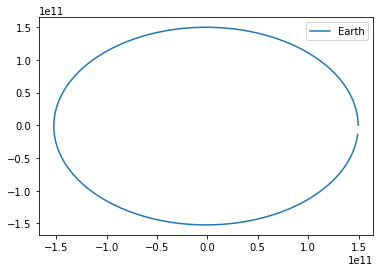
\includegraphics[width=7cm]{figure1.png} }}%
    \qquad
    \subfloat[\centering General n = 100]{{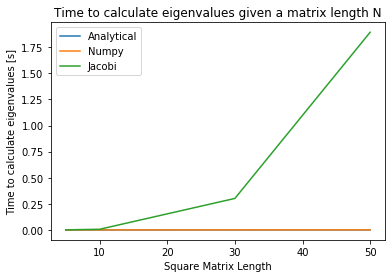
\includegraphics[width=7cm]{figure2.png} }}%
    \caption{Comparison between the general Thomas Algorithm for n = 10 and 100 respectively}%
    \label{fig:1}%
\end{figure}
\break
We can see that even for $n = 100$ we don't get a perfect fit.
Compare this to the special solution for the Thomas Algorithm, which you can see in Figure \ref{fig:2} below.
We see that the special solution is a much better fit already and we're only using $n = 100$.
Additionally, if we count the FLOPs of our program manually, we'll find that the general solution uses 9 FLOPs throughout it's loops. Comparatively, the specialized solutions cuts this down to 4 FLOPs, since the algorithm runs $n-1$ times, we get:
\begin{equation*}
FLOPs_{gen} = 9(n-1) = 9n
\end{equation*}
\begin{equation*}
FLOPs_{spec} = 4(n-1) = 4n
\end{equation*}
We've gauged the accuracy of our model using equation \ref{6}, which gives us (Figure \ref{fig:3}):
\break
\begin{figure}
    \centering
    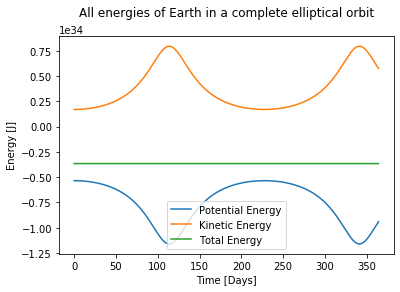
\includegraphics[width=0.5\textwidth]{figure8.png}
    \caption{Relative Error given a timestep h}
    \label{fig:3}
\end{figure}
We see that (maybe unsurprisingly) given a smaller stepsize we get more accurate results. The only exception is a sudden jump for $n=10^6$ which I can't explain. Maybe a rounding error?
\begin{figure}[hbt!]
    \subfloat[\centering Special n = 10]{{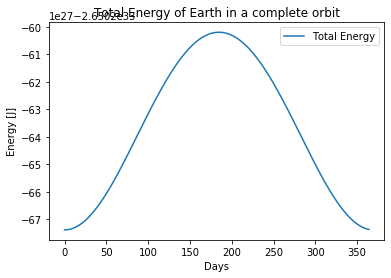
\includegraphics[width=7cm]{figure4.png} }}%
    \qquad
    \subfloat[\centering Special n = 100]{{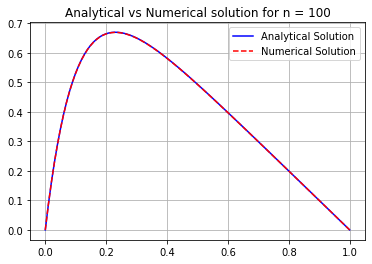
\includegraphics[width=7cm]{figure5.png} }}%
    \caption{Comparison between the special Thomas Algorithm for n = 10 and 100 respectively}%
    \label{fig:2}%
\end{figure}
\break
Lastly we tried to solve the same problem with an LU decomposition. Above you'll find a table with the results (table \ref{tab:1}) and a complimenting plot below (figure \ref{fig:4})
\begin{table}[hbt!]
    \centering
    \begin{tabular}{c|c|c}
         General [s]& Special [s]& LU [s] \\
         $2.7\times 10^{-5}$& 0.0088& 0.098 \\
         0.0002& 0.0088& 0.00049 \\
         0.002& 0.0097& 0.016 \\
         0.0211 & 0.019& 9.3 \\
         0.21 & 0.24& --- \\
         2.0 & 1.1& --- \\
         20 & 11& --- \\
    \end{tabular}
    \caption{Runtimes for every method in seconds}
    \label{tab:1}
\clearpage
\end{table}
\begin{figure}[h]
    \centering
    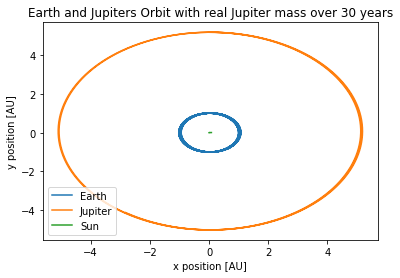
\includegraphics[width=0.5\textwidth]{figure7.png}
    \caption{Time taken to run algorithm given a power of n}
    \label{fig:4}
\end{figure}
We see that LU-decomposition isn't viable for big matrices, but it works very well and is by far the easiest to implement for small matrices. There are no measurements past $n=100000$ because that would require more memory than I have.
\section{Discussion}
The first thing I'd like to discuss is error. I decided not to add error bars and find the average of benchmark times given that I had incredibly small deviances, with only a few outliers, which we're not supposed to include anyway.
Secondly I'd like to discuss the equations \ref{10} and \ref{11}. I realized this a bit too close to the deadline to act on it, but I could've saved a FLOP if I had combined $\frac{a_{i-1}}{\Tilde{b_i}}$ and made them into some variable C as such:
\begin{equation*}
    C=\frac{a_{i-1}}{\Tilde{b_i}}
\end{equation*}
So in actuality, we're going from 8n FLOPs to 4n when specializing our algorithm.
Thirdly I'd like to discuss in a bit more detail the difference between LU-decomposition and the Thomas Algorithm. The primary reason why we're able to get away with much larger numbers should we TDMA is that we're only ever storing three vectors, as opposed to LU which requires an entire matrix. For our limit, $n=100000$, we'd have a matrix with a size of $100000\times 100000$. Given that floats in Python are double precision floats, every number will individually require 8 bytes, which would be $8 \times 10^{10}$ bytes, or 80Gb, much more than I or any other commercially available computer has, unless you're a rather eccentric enthusiast.

\section{Conclusion}
In conclusion, we've shown and calculated the solution of the one dimensional Poisson Equation. We've used both a TMAD and an LU-decomposition, and weighted them against each other. We've also shown that, in some specific cases, you can optimize your TMAD for upto (in our case) a 100\% increase in computing speed, from 8n FLOPs to 4n. We've also shown the limitations of LU-decomposition and the importance of effectivizing your algorithm to save memory (and time) when working on larger data sets.
\section{Sources}
M.Hjorth-Jensen, FYS3150/FYS4150 Lecture Notes 2020, 2020
\end{document}
